\ifx\ucebnice\undefined
\documentclass[a5paper,10pt,twoside]{book}
\usepackage{luatex85}
\usepackage{latexsym}
\usepackage{amsmath}
\usepackage{amsfonts}
\usepackage{amsthm}
\usepackage{amssymb}
\usepackage{fncylab}
\usepackage{comment}
\usepackage{float}
\usepackage{wrapfig}
\usepackage{tikz}
\usepackage{tikz-qtree}
\usepackage{url}
\usepackage{xcolor}
\usepackage{pdfpages}
\usepackage[czech]{babel}
\definecolor{svlinks}{rgb}{.0,0.3,0.6} %tmavě modrá
\usepackage[bookmarks, colorlinks=false,pdfhighlight=/O,linkcolor=svlinks,urlcolor=svlinks,
            pdftitle={Úvod do programování (část II: Algoritmy},
            pdfauthor={Jonathan L. Verner},
            pdfsubject={Algoritmy a složitost},
            pdfkeywords={algoritmus, složitost, Python, třídění, grafy},
            bookmarksdepth=3
            ]{hyperref}
\usepackage[toc,xindy,nopostdot,nonumberlist]{glossaries}
\usepackage[top=2cm,bottom=2cm,left=2cm,right=1cm]{geometry}
\usepackage{fancyhdr}
\usetikzlibrary{decorations.fractals,chains,fit,shapes,patterns}
% \usepackage[utf8]{inputenc}
% \usepackage[T1]{fontenc}
% \usepackage{palatino}
\usepackage{unicode-math}
\usepackage{fontspec}
\usepackage{attachfile}
\usepackage{minted}
\usepackage{multicol}
\usepackage{caption}
\usepackage{titlesec,titletoc}
\usepackage[letterspace=150]{microtype}
\relpenalty=9999
\binoppenalty=9999


% \ifblackandwhite
%   \newcommand{\logoUK}{\includegraphics[width=20mm]{UK-logo}}
%   \definecolor{UKRed}{RGB}{0,0,0}
%   \definecolor{Gray}{RGB}{0,0,0}
% \else
  \newcommand{\logoUK}{\includegraphics[width=20mm]{UK-logo-red}}
  \definecolor{UKRed}{RGB}{210,45,64}
  \definecolor{Gray}{HTML}{5e6a71}
% \fi

%----------definitions---------------------------


%math definitions

\newcommand{\R}{\mathbb R}
% \newcommand{\C}{{\mathcal C}}
\newcommand{\F}{{{\mathcal F}}}
% \newcommand{\U}{{{\mathcal U}}}
\newcommand{\V}{{{\mathcal V}}}
\newcommand{\cont}{{\mathfrak{c}}}
\newcommand{\force}{\Vdash}
\newcommand{\pw}{{{\mathcal P}}}
\newcommand{\MU}{{\mathbb{M}_{\mathcal{U}}}}
\newcommand{\pomega}{\pw(\omega)}


\newcommand{\src}[3][]{%
\begin{program}%
\caption{#3\hfill%
\attachfile[author={Jonathan Verner},
            description={Source code for #3},
            mimetype={text/x-python},
            print=false,
            color=1 1 1,
            icon={Tag}]{kod/#2.py}}
\label{alg:#2}{\inputminted[linenos]{python}{kod/#2.py}}
\end{program}}


\newcommand{\srcsplit}[4][]{%
\begin{program}%
\caption{#3\hfill%
\attachfile[author={Jonathan Verner},
            description={Source code for #3},
            mimetype={text/x-python},
            print=false,
            color=1 1 1,
            icon={Tag}]{kod/#2.py}}
\label{alg:#2}{\inputminted[linenos,lastline=#4]{python}{kod/#2.py}}
\end{program}
\begin{program}%
\caption*{#3\hfill%
(pokračování algoritmu \ref{alg:#2})}
\inputminted[linenos,firstline=#4]{python}{kod/#2.py}
\end{program}
}

\newcommand{\sniphere}[1]{%
\label{alg:#1}\inputminted[linenos]{python}{kod/#1.py}
}

\newcommand{\srchere}[3][]{%
\begin{programhere}%
\caption{#3\hfill%
\attachfile[author={Jonathan Verner},
            description={Source code for #3},
            mimetype={text/x-python},
            print=false,
            color=1 1 1,
            icon={Tag}]{kod/#2.py}}
\label{alg:#2}\inputminted[linenos,#1]{python}{kod/#2.py}
\end{programhere}}


\newcommand{\varsrc}[3][]{%
\begin{program}%
\caption{#3\hfill%
\attachfile[author={Jonathan Verner},
            description={Source code for #3},
            mimetype={text/x-python},
            print=false,
            icon={Paperclip}]{kod/#2.py}}
\label{alg:#2}\inputminted[linenos]{python}{kod/#2.py}
\end{program}}



 %% ALGORITHMS
 \floatstyle{ruled}
 \newfloat{program}{htbp}{listings}[chapter]
 \newfloat{programhere}{H}{listings}[chapter]
 \floatname{program}{Algoritmus}
 \floatname{programhere}{Algoritmus}

 % Make program and programhere share counters
% (LaTeX constructs a counter by prepending the float-name with c@
 \makeatletter
 \let\c@programhere\c@program
 \makeatother

 %---------numbering of the theorems------------
 \swapnumbers

 \newtheorem*{theorem*}{Věta}
 \newtheorem{theorem}[program]{Věta}
 \newtheorem{example}[program]{Příklad}
 \theoremstyle{definition}
 \newtheorem{definition}[program]{Definice}
 \newtheorem{question}[program]{Problém}
 \newtheorem{uloha}[program]{Úloha}
 \newtheorem{cviceni}[program]{Cvičení}
 \newtheorem{cviceniH}[program]{Cvičení (*)}
 \newtheorem*{reseniIMPL*}{Řešení}
 \specialcomment{reseni}{\begin{reseniIMPL*}}{\end{reseniIMPL*}}
 \excludecomment{reseni}
 \excludecomment{todo}
 \newtheorem*{comments*}{Komentáře}
 \newtheorem*{definition*}{Definice}
 \newtheorem{remark}[program]{Poznámka}
 \newtheorem*{note}{Poznámka}


% GLOSSARIES

\newglossary{person}{gls}{glo}{Lidé}
\DeclareRobustCommand{\textemph}[1]{\emph{#1}}
\renewcommand{\glsdisplay}[4]{\textemph{#1 (\glsentryuseri{\glslabel})}}
\newcommand{\person}[2][]{\gls{person:#2}}
\newenvironment{doplneni}{%
\par
\leftskip1cm
\rightskip1cm
\small
}{\par}

\newenvironment{python}{%
 \VerbatimEnvironment
 \begin{minted}[linenos]{python}}
{%
\end{minted}%
}

\loadglsentries[person]{people.tex}
\makeglossaries
% \printglossary[type=person,title={Lidé}]

 \hypersetup{
    colorlinks,%
    citecolor=black,%
    filecolor=black,%
    linkcolor=black,%
    urlcolor=black
}

% \pdfinfo{
%       /Author (Jonathan Verner)
%       /Title (ALG110006 Úvod do programování: Poznámky k přednášce, LS)
%       /Subject (programování, algoritmy)
%       /Keywords (quicksort,heapsort,dijsktra,graph,euclid)
%    }



% Chater & Section title formatting (uses the titlesec package)
\titleformat{\chapter}[block]{\sf\Huge\raggedright}{\hskip-1cm{\color{UKRed}\thechapter\hskip5mm\vrule}}{1em}{}
\titleformat{\section}[block]{\sf\Large}{\hskip-1cm{\color{UKRed}\thesection}}{3.5mm}{}

% Table of contents formatting
\titlecontents{chapter}
[0pt]
{\addvspace{1pc}}
{\contentsmargin{0pt}%
\makebox[0pt][r]{\sf\color{UKRed}\large\thecontentslabel\enspace}%
\sf\large}
{\contentsmargin{0pt}%
\large}
{\hfill\quad\sf\thecontentspage}
[\addvspace{2mm}]

\titlecontents{section}
[7mm]
{}
{\contentsmargin{10pt}%
\makebox[0pt][r]{\sf\color{UKRed}\thecontentslabel\enspace}%
\sf}
{\contentsmargin{10pt}}
{\hfill\quad\sf\thecontentspage}
[]



% Table of contents has two-column layout with a 2cm gap
% Note that the following can lead to conflicts with some packages
% which aggressively want to execute code AtEnd and AtBegin
% \columnsep=2cm
% \AtBeginDocument{\addtocontents{toc}{\protect\begin{multicols*}{2}}}
% \AtEndDocument{\addtocontents{toc}{\protect\end{multicols*}}}



\setsansfont{gill-sans-mt}
\setmainfont[Ligatures={Common,Rare,Historic,TeX}]{Caladea}
\setmathfont{cambria-math}
\setmonofont{Inconsolata}
\newfontfamily\Bodoni{Libre Bodoni}

%-------------opening--------------------------
\begin{document}
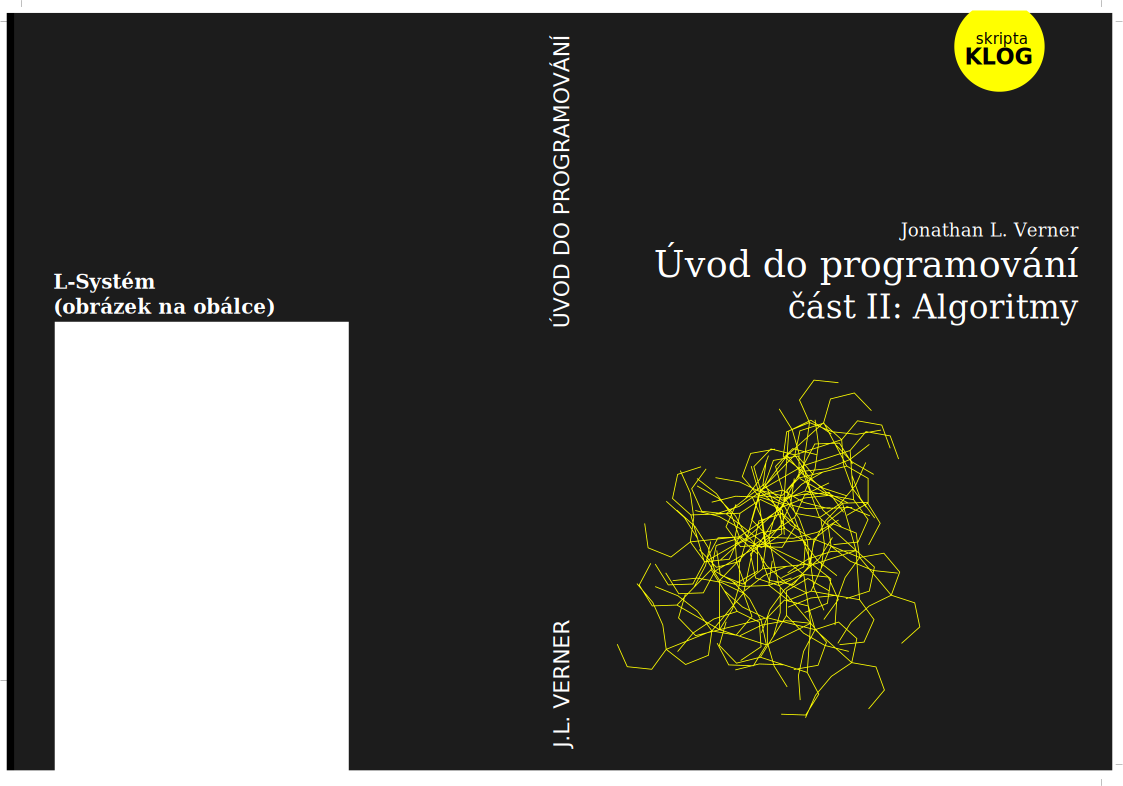
\includepdf[pages={1},noautoscale=true,fitpaper=true,offset=-8cm 0]{obalka-black.pdf}


\title{}

% \author{Jonathan Verner}
% \address{Department of Logic, Charles University\\
% Palachovo nám. 2\\ 116 38 Praha 1, Czech Republic}
% \email{jonathan.verner{@}ff.cuni.cz}
%\thanks{The author was partially supported by }

%\subjclass[2010]{Primary }
%\keywords{}

%\begin{abstract}
%\end{abstract}
%\maketitle
% \pagestyle{empty}

\headheight=12.4pt
\pagestyle{fancy}

%\hsize=16cm
\parindent=0cm
\parskip=0.2cm
\thispagestyle{empty}
\
\vskip1cm
Jonathan L. Verner, PhD.\\
Katedra Logiky\\
Filozofická fakulta UK\\
Palachovo náměstí 2\\
116 18 Praha 1
\vfill
\copyright\ Jonathan L. Verner, 2015 \\[3mm]
{\small Tato učebnice slouží jako skripta k letnímu semestru přednášky
\emph{Úvod do programování}, vypsané pod kódem ALG110006 na Katedře logiky FF UK
v letech 2011--2015. Jejich příprava byla podpořena projektem
OPVK CZ.1.07/2.2.00/28.0216 \emph{Logika: systémový rámec rozvoje oboru v ČR a
koncepce logických propedeutik pro mezioborová studia}\\}


\includegraphics[width=12cm]{logolink}
\eject
\thispagestyle{empty}
\
\vskip3cm
\begin{center}
 \sf\Huge Úvod do programování\\[1cm]
 \sf\Large část II: Algoritmy
\end{center}
\vfill
\eject

\lhead[\sf{\bf\thepage}]{\sf\nouppercase{\leftmark}}
\rhead[\sf\nouppercase{\leftmark}]{\sf\bf\thepage}
\cfoot{}

\tableofcontents

\setcounter{section}{5}
\fi
\section{Složitost podruhé}
V předchozích kapitolách jsme se setkali s výběrem některých typických úloh, se kterými
se programátoři setkávají. Ke každé takové úloze jsme si ukazovali i postup, jak jí vyřešit
a zkoumali efektivnost tohoto postupu. Pro většinu úloh jsme nalezli řešení, které bylo
z mnoha hledisek efektivní, nicméně občas jsme zmínili (vzpomeňte třeba
úlohu \ref{uloha:minimalcoloring}, kde šlo o nalezení optimálního obarvení grafu), že 
efektivní postup není znám a naznačili jsme, že možná ani neexistuje. Nyní se
budeme tímto problémem zabývat podrobněji. 

Když bychom na chvíli zapomněli na efektivnost, mohli bychom alespoń doufat, že každý problém, na který
narazíme, bude mít nějaké --- třeba i velmi neefektivní --- řešení. Ukážeme si, že tato naděje
je planá. Existují totiž i velmi jednoduché a prakticky zajímavé problémy, které neumíme
vyřešit žádným algoritmem. A to nikoliv protože bychom nebyli dostatečně vynalézaví, ale protože
žádný algoritmus, který by úlohu řešil, neexistuje. Hned si jednu takovou úlohu ukážeme. Když jsme 
se učili pracovat s rekurzí, bylo třeba dát pozor, abychom ošetřili základní případy. Jinak by 
došlo k tomu, že by se program do nekonečna zacyklil. Podobný problém nastává u while cyklů, 
pokud si nedáme pozor na cyklící podmínku. Asi každému bude na první pohled jasné, že následující 
program nikdy neskončí, protože se zacyklí:

\begin{python}
i=0
while True:
   i = i * i 
\end{python}

Poněkdu zákeřnější může být funkce, která zdánlivě počítá faktoriál:

\begin{python}
def bad_factorial(n):
    ret = 1
    while n != 1:
        ret *= n
        n = n - 1
    return ret
\end{python}

Funkce možná vypadá správně, ale zkuste si rozmyslet, co se stane, když se pomocí ní pokusím spočítat
faktoriál 0. Nejen, že nespočítá správný výsledek 1, ona totiž nespočítá vůbec žádný výsledek ---
do nekonečna se zacyklí! Zkušenější programátor uvidí chybu okamžitě, ale asi si dokážeme představit,
že u složitějšího kódu, který bude mít třeba desítky tisíc řádků, už bude chybu hledat velmi dlouho.
Bylo by proto výhodné, kdyby mu práci usnadnil počítač. To vede k následující úloze:

\begin{uloha}\label{uloha:halting-problem} Pro zadaný program a vstupní data určete, zda se program zastaví, nebo se zacyklí.
\end{uloha}

Když bychom se pustili do řešení, asi bychom se snažili nejprve najít všechny while cykly a nějak analyzovat
podmínky, za kterých se cyklus ukončí. Naše funkce by mohla vypadat třeba takto:

\begin{python}
def zacykli( funkce, parametry ):
    """ Vrátí true, pokud se příkaz 
    
         funkce(parametry)
       
        zacyklí. V opačném případě vrátí False.
    """
    ...
\end{python}

Zbývá už jen doplnit zmíněnou analýzu cyklů... Řekněme, že by se nám to povedlo a zkusme se podívat na následující
příklad:

\begin{python}
def priklad():
    if zacykli(priklad, None):
        return 0
    else:
        while True:
          i = 1
\end{python}

Funkce {\tt priklad} vypadá trochu podezřele. V prvním kroku použije naší důmyslnou funkci {\tt zacykli} a
zeptá se, co si myslí o volání funkce {\tt priklad}. Pokud je odpovědí, že se zacyklí, pak funkce
{\tt priklad} vrátí 1. V opačném případě se zacyklí. Na tomto slovním popisu je už asi vidět, že ta
podezřelost je oprávněná, někde dojde k problémům. Co se stane, když nyní na tuto funkci aplikujeme
{\tt zacykli}? Dostaneme špatnou odpoveď! Pokud totiž bude odpoveď True, mělo by to znamenat, že funkce
{\tt priklad} se zacykli. Jenže když si jí projdeme, pak zjistíme, že se nemohla zacyklit, protože
skončila na řádku 3 vrácením 0. No dobrá, tak tedy odpověď musí být False, což má znamenat, že se
funkce {\tt priklad} nezacyklí. Ale ouha, to je zase špatně --- v tomto případě se totiž funkce {\tt priklad}
dostane na řádek 5 a nenávratně se zacyklí.












\begin{todo}
\subsection{Reprezentace aritmetických výrazů}
\paragraph{Stromová reprezentace}
\paragraph{Infixová notace}
\paragraph{Prefixová a postfixová notace}
\subsection{Převádění mezi notacemi}
\subsection{Vyhodnocování}
\end{todo}
\ifx\ucebnice\undefined
\renewcommand{\refname}{\textbf{Literatura}}
\bibliographystyle{mujstyl}
\bibliography{ref}
\renewcommand{\glossarypreamble}{Biografické údaje jsou převzaté z \href{http://www.wikipedia.org}{Wikipedie}.}
\printglossary[type=person,title={Lidé}]
\end{document}
\fi
